\documentclass[a4paper,twoside]{article}

\usepackage{epsfig}
\usepackage{subcaption}
\usepackage{calc}
\usepackage{amssymb}
\usepackage{amstext}
\usepackage{amsmath}
\usepackage{amsthm}
\usepackage{multicol}
\usepackage{pslatex}
\usepackage{apalike}
\usepackage[bottom]{footmisc}
\usepackage{SCITEPRESS}     % Please add other packages that you may need BEFORE the SCITEPRESS.sty package.

\usepackage{algorithm}
%\usepackage{algorithmic}
\usepackage{algpseudocode}

%
% These are are recommended to typeset listings but not required. See the subsubsection on listing. Remove this block if you don't have listings in your paper.
\usepackage{newfloat}
\usepackage{listings}
\lstset{%
	basicstyle={\footnotesize\ttfamily},% footnotesize acceptable for monospace
	numbers=left,numberstyle=\footnotesize,xleftmargin=2em,% show line numbers, remove this entire line if you don't want the numbers.
	aboveskip=0pt,belowskip=0pt,%
	showstringspaces=false,tabsize=2,breaklines=true}
\floatstyle{ruled}
\newfloat{listing}{tb}{lst}{}
\floatname{listing}{Listing}


\usepackage{caption}
\usepackage{subcaption}

\usepackage{multirow}

\usepackage{footmisc}

\usepackage{amsthm}
\usepackage{amsmath}
% \usepackage{amssymb}
\usepackage{url}\urlstyle{tt}

\usepackage{listings}
\lstdefinelanguage{clingo}{%
  keywordstyle=[1]\usefont{OT1}{cmtt}{sb}{n},%
  keywordstyle=[2]\textbf,%
  keywordstyle=[3]\usefont{OT1}{cmtt}{m}{n},%
  alsoletter={\#,\&},%
  keywords=[1]{not,from,import,def,if,else,elif,return,while,break,and,or,for,in,del,and,class,with,print,as,is},%
  keywords=[2]{\#const,\#show,\#minimize,\#base,\#theory,\#count,\#external,\#program,\#script,\#end,\#heuristic,\#edge,\#project,\#show,\#sum},%
  keywords=[3]{&,&dom,&sum,&diff,&show},%
  literate=~{$\sim$}2,%
  morecomment=[l]{\#\ },%
  morecomment=[l]{\%\ },%
  morestring=[b]",%
  stringstyle={\textit},%
  commentstyle={\color{darkgray}}%
}
\lstset{%
  numbers=left,
  numberblanklines=false,
  basicstyle=%
  \ttfamily%
  \lst@ifdisplaystyle\scriptsize\fi,
  language=clingo}
\lstset{escapeinside={*@}{@*}}
% Fix for twocolumn margins
\lstset{%
  xleftmargin=5mm,
  framexleftmargin=5mm}
  
\newtheorem{prop}{Proposition}

% = Custom Macros ==================================================================================

% - MAPF -------------------------------------------------------------------------------------------

\newcommand{\inst}{\ensuremath{\mathcal{M}}}
\newcommand{\gex}[1]{\ensuremath{\mathsf{gex}_{#1}}}
\newcommand{\mrelax}[3]{\ensuremath{{#1}_{#2,#3}}}
\newcommand{\rstart}{\operatorname{start}}
\newcommand{\rdest}{\operatorname{dest}}
\newcommand{\makespan}{\ensuremath{\mathrm{ms}}}

\newcommand{\mrelaxle}{\ensuremath{\mathrel{\prec_{relax}}}}

% - asprilo ----------------------------------------------------------------------------------------

\newcommand{\Mdom}{\textbf{M}}

% - logical formulas -------------------------------------------------------------------------------

\newcommand{\dneg}{\ensuremath{\sim\!}}

% - corridor ---------------------------------------------------------------------------------------

\newcommand{\ssb}{\ensuremath{\mathbf{B}}}
\newcommand{\ssc}{\ensuremath{\mathbf{C}}}
\newcommand{\ssm}{\ensuremath{\mathbf{M}}}
\newcommand{\ssp}{\ensuremath{\mathbf{P}}}

\newcommand{\pss}{\ensuremath{\mathbf{SP}}}
\newcommand{\psa}{\ensuremath{\mathbf{AP}}}
\newcommand{\psr}{\ensuremath{\mathbf{RP}}}
\newcommand{\psd}{\ensuremath{\mathbf{DP}}}

%%% Local Variables:
%%% mode: latex
%%% TeX-master: "main"
%%% End:


\begin{document}

\title{Multi-agent Pathfinding on Large Maps Using Graph Pruning:\\This Way or That Way?}

%\author{Paper \#41}


\author{
\authorname{Jiří Švancara\sup{1}\orcidAuthor{0000-0002-6275-6773}, Philipp Obermeier\sup{2,}\sup{3}\orcidAuthor{0000-0001-6346-4855}, Matej Husár\sup{1}, Roman Barták\sup{1}\orcidAuthor{0000-0002-6717-8175} and Torsten Schaub\sup{2,}\sup{3}\orcidAuthor{0000-0002-7456-041X}}
\affiliation{\sup{1}Charles University, Prague, Czech Republic}
\affiliation{\sup{2}University of Potsdam, Potsdam, Germany}
\affiliation{\sup{3}Potassco Solutions, Potsdam, Germany}
\email{svancara@ktiml.mff.cuni.cz, phil@cs.uni-potsdam.de, husarmatej@gmail.com, bartak@ktiml.mff.cuni.cz, torsten@cs.uni-potsdam.de}
}


\keywords{Multi-agent Pathfinding, Answer set programming, Subgraph, Shortest path}

\abstract{Multi-agent pathfinding is the task of navigating a set of agents in a shared environment from their start locations to their desired goal locations without collisions. Solving this problem optimally is a hard task and various algorithms have been devised. The algorithms can be in general split into two categories -- search-based and reduction-based. It is known that reduction-based algorithms struggle with large instances in terms of the size of the map (shared environment). A recent study tried to mitigate this drawback by pruning some vertices of the map. The pruning is done based on the vicinity to a shortest path of an agent. In this paper, we study the effect of choosing such shortest paths. We provide several approaches to choosing the paths and we perform an experimental study to see the effect on the runtime.}

\onecolumn \maketitle \normalsize \setcounter{footnote}{0} \vfill

\section{Introduction}

In this paper, we study the problem of Multi-agent pathfinding (MAPF). The task is to navigate a set of agents in a shared environment (map) from starting locations to the desired goal locations such that there are no collisions~\cite{DBLP:conf/aiide/Silver05}. This problem has numerous practical applications in robotics, logistics, digital entertainment, automatic warehousing and more, and it has attracted significant focus from various research communities in recent years~\cite{sven_lifelong,DBLP:conf/ijcai/Surynek19,ngobsoscye17a,geobscra18a}.

The optimal MAPF solvers can be in general split into two categories -- search-based and reduction-based. The former algorithms search over possible locations or conflicts among the agents, the latter reduce the problem to some other well-defined formalism such as Answer Set Programming (ASP)~\cite{geobotscsangso18a}. While it is not always the case, it is generally established that each of the approaches dominates on different types of instances~\cite{DBLP:journals/access/GomezHB21,DBLP:conf/icaart/SvancaraB19}. The search-based solvers are easily able to find solutions on large sparsely populated maps while having trouble dealing with small densely populated maps. On the other hand, the reduction-based solvers are able to deal with the small densely populated maps but are unable to find a solution for large maps even with a small number of agents.

\subsection{Contributions}

Since the reduction-based solvers have trouble solving instances on large maps, a recent study~\cite{AAMAS_corridors} proposed techniques to prune the map of vertices that are most likely not needed to solve the instance. The pruning is done based on a random shortest path for each agent. Only the vertices around the selected path are considered and the other vertices are removed from the instance, creating a much simpler problem. In this paper, we extend the original study by examining the behavior of the technique by using more than just one shortest path for each agent. First, we describe the four strategies of pruning the graph (map) from the original study, then we introduce the four new approaches to select the paths for each agent as a novel contribution of this paper.

%\subsection{Structure of the paper}

%The paper is structured as follows. First, we establish formal definitions used in MAPF, then we introduce the ASP encoding we used as our reduction-based MAPF solver. In section~\ref{sec:subgraph}, we describe the sub-graph method from~\cite{AAMAS_corridors}. In section~\ref{sec:SP}, we describe our contribution of choosing the shortest paths for each agent. Lastly, we perform experimental evaluation of all of the different approaches.
\section{Definitions}

\emph{MAPF instance} $\inst$ is a pair $\inst = (G,A)$, where $G$ is a graph $G = (V,E)$ and $A$ is a set of agents. Each agent $a_i \in A$ is a pair $a_i = (s_i,g_i)$, where $s_i \in V$ is a starting location and $g_i \in V$ is a goal location of agent $a_i$.

Our task is to find a \emph{valid plan} $\pi_i$ for each agent $a_i \in A$ such that it is a valid path from $s_i$ to $g_i$. We use $\pi_i(t) = v$ to denote that agent $a_i$ is located in vertex $v$ at timestep $t$. Time is discrete and at each timestep $t$, an agent can either wait in its current location or move to a neighboring location.

Furthermore, we require that each pair of plans $\pi_i$ and $\pi_j$, $i \neq j$ is collision-free. Based on MAPF terminology~\cite{stern2019mapfVarians}, there are five types of collisions. % (see Figure~\ref{fig:conflict_def}). 
In this work, we forbid \emph{edge}, \emph{vertex}, and \emph{swapping} conflict while allowing \emph{following} and \emph{cycle} conflicts since during the last two conflicts, the agents are not occupying the same physical location. Note however, that all of the proposed methods will work with any other setting as well.%We call this setting \emph{parallel motion}, as opposed to \emph{pebble motion}~\cite{pebble_motion}, where all of the conflicts are forbidden.

%\begin{figure}[ht]
%\centering
%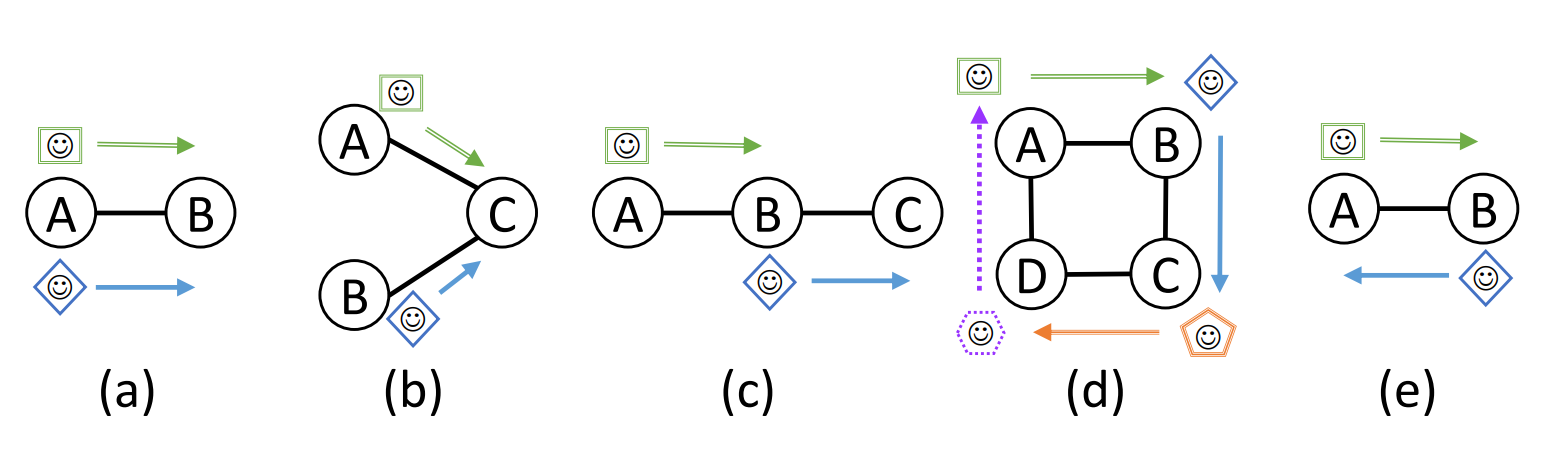
\includegraphics[width=0.99\columnwidth]{img/conflicts.PNG}
%\caption{Conflicts between two or more agents. (a) \emph{edge conflict}, (b) \emph{vertex conflict}, (c) \emph{following conflict}, (d) \emph{cycle conflict}, (e) \emph{swapping conflict}. Figure taken from~\cite{stern2019mapfVarians}.}
%\label{fig:conflict_def}
%\end{figure}

In this paper, we are interested in finding a \emph{makespan} optimal solution. Makespan (or sometimes horizon) is the temporal duration of the plan. Once an agent arrives at its goal location it does not disappear. It may move out of the goal location again, however, the plan ends once all of the agents are at the goal location at the same time. This means that the length of the plan $|\pi_i|$ is the same for all of the agents. Another cost function often used in literature is \emph{sum of costs}~\cite{ICTS_soc}. Note that finding an optimal solution for either of the cost functions is an NP-Hard problem~\cite{NP-hard1,NP-hard2}.
\section{ASP Encoding}

%
% - Action theory ----------------------------------------------------------------------------------
%
% To describe both movement actions and positional changes of agents,
We use an ASP encoding%
%
\footnote{% can we make this a citation?
 \url{https://github.com/potassco/asprilo-encodings/blob/master/m/action-M.lp}}
%
for MAPF % in Listing~\ref{enc:action},
due to~\cite{geobotscsangso18a}.
The encoding assumes a grid graph \(G\) and plans agents in parallel within a makespan while avoiding conflicts.
%
Specifically,
the plan's timesteps are bound by the makespan $H$. % in Line 1.
%
%Line~3 gives the four cardinal directions,
%used in Line~4 to represent all transitions on the grid with its x,y-coordinates stated by predicate~\lstinline{position/1}.
%%
%Possible movement actions, at most one per agent and timestep, are generated by Line~8.
%%
%Related preconditions and positional changes are described in Lines~10-12:
The positions of all agents are described by \lstinline{position(R,C,T)} stating that agent \lstinline{R} is at x,y-coordinates \lstinline{C} at time \lstinline{T}.
Constraints are added to ensure the correct movement of the agents as well as collision avoidance.
%
%For an agent \lstinline{R} sitting idle at time \lstinline{T},
%the frame axiom in Lines 14-15 propagates its unchanged position.
%
%Swapping conflicts are prevented by Lines~17-19, and both edge and vertex conflicts by Line 21.
%
% ----------------------------------------------------------------------------------------------
%\lstinputlisting[
%floatplacement=ht,
%label=enc:action,
%linerange={4-24},
%captionpos=b,
%caption={Action theory for agent movements.}
%]{listings/asp/action-M.lp}
% ----------------------------------------------------------------------------------------------
%
%
% - Goal condition, assignment, TGE ------------------------------------------------------------
%
Further,
we
% augment the action theory encoding with the goal condition %in Listing~\ref{enc:goal} to
enforce that every agent \lstinline{R} has reached its goal coordinates \lstinline{C}, stated by \lstinline{goal(R,C)},
at the time $H$.
%
% ----------------------------------------------------------------------------------------------
%\lstinputlisting[
%floatplacement=ht,
%label=enc:goal,
%linerange={2-2},
%captionpos=b,
%caption={Goal condition for agents and assigned nodes.}
%]{listings/asp/assigned-goal.lp}
% ----------------------------------------------------------------------------------------------
%
%Overall,
%our ASP encoding consists of the action theory (Listing~\ref{enc:action}) in conjunction with the goal condition (Listing~\ref{enc:goal}) and expects an MAPF instance in form of the aforementioned ASP facts as input.
%

There are two common techniques to speed up computation. First, using a lower bound for the makespan. % instead of starting with $H = 1$
A simple lower bound is to compute for each agent $a_i$ the shortest path from its start location $s_i$ to its goal location $g_i$. The lower bound for $H$ is then the longest of these shortest paths. % It is often the case that this lower bound is actually the optimal solution.
%
Another enhancement is to pre\-pro\-cess the variables representing agent locations. These variables correspond to an agent being present at some location at a time. However, for some locations, the specific agent cannot be present at the specific times. % , because it needs to be present at times $0$ and $H$
Specifically, for agent $a_i$, if vertex $v$ is distance $d$ away from start location $s_i$, we know that the agent $a_i$ cannot be at vertex $v$ at times $0,\dots,(d-1)$. % because it cannot travel the distance in time
Similarly, if vertex $v$ is distance $d$ away from goal location $g_i$, agent $a_i$ cannot be present at vertex $v$ at times $H-d+1,\dots,H$. %We add the integrity constraint in Listing~\ref{enc:possloc} to ensure that agent \lstinline{R} occupies an eligible position \lstinline{C} at time \lstinline{T}, expressed by a fact \lstinline{poss_loc(R,C,T)}.
%
% ----------------------------------------------------------------------------------------------
%\lstinputlisting[
%floatplacement=ht,
%label=enc:possloc,
%linerange={3-4},
%captionpos=b,
%caption={Eligible agent locations from pre-processing.}
%]{listings/asp/possible_location.lp}
% ----------------------------------------------------------------------------------------------
% done
%\com{PO: mby describe how this is facilitated in SAT?}

\section{The Sub-Graph Method}
\label{sec:subgraph}

\subsection{Motivation}


Both of the improvements mentioned in the last section maintain completeness and optimality. However, there are situations, where too many possibilities for the agent's location remain, which may overwhelm the underlying solver. The motivation from~\cite{AAMAS_corridors} can be seen in Figure~\ref{fig:diagonal}. The agent is placed on a 4-connected grid map going from one corner to the diagonally opposite corner. With just one agent and no obstacles, there are $\binom{2(N-1)}{N-1}$ possible shortest paths if the size of the grid is $N \times N$. As seen in the figure, the preprocessing correctly finds at what timesteps the agent can be located at which vertices. However, the number of choices for the solver is still too large. The proposition is to pick just one of the shortest paths and treat the other vertices as an impassable obstacle. Hence, for these vertices, there are no variables entering the solver. Such pruning of the graph can be seen in Figure~\ref{fig:diagonal_path}.

\begin{figure}[ht]
\centering
\hspace{0.9cm}
\begin{subfigure}{0.27\columnwidth}
\centering
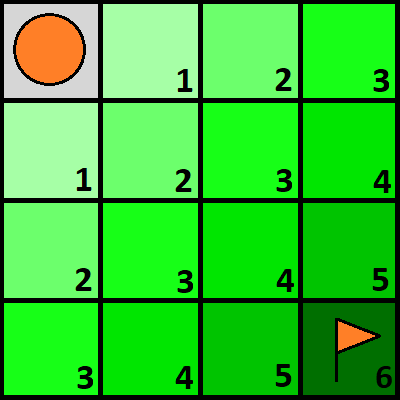
\includegraphics[width=\textwidth]{img/diagonal_agent.png}
\caption{}
\label{fig:diagonal}
\end{subfigure}
\hfill
\begin{subfigure}{0.27\columnwidth}
\centering
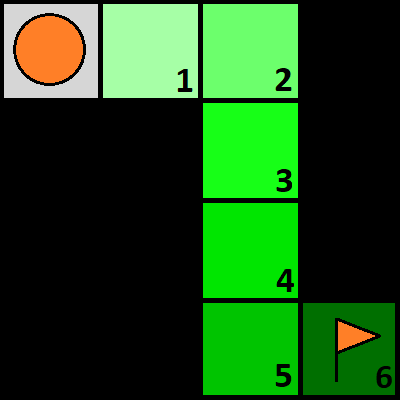
\includegraphics[width=\textwidth]{img/diagonal_single_path.png}
\caption{}
\label{fig:diagonal_path}
\end{subfigure}
\hspace{0.9cm}
\caption{An agent moving on a grid map from a corner to the opposite one. The numbers represent at what timesteps the agent can reach the given vertex.}
\label{fig:diagonal_example}
\end{figure}


%Another example where this approach is helpful can be seen in Figure~\ref{fig:two_agents}. The two agents have different lengths of shortest paths. For the orange agent with the longer path, preprocessing correctly finds the only shortest path. However, the blue agent with a much shorter path may move anywhere in the shaded area since it has enough time. Recall that we are computing makespan optimal solutions, so we are interested in the timestep when all agents are at their goal locations. This time is prolonged by the orange agent, therefore the blue agent has many more choices. If we use our pruning technique the number of choices reduces dramatically. The blue agent can still choose when to move to the goal location, or even move back and forth a few times, however, it may use significantly fewer vertices.

%\begin{figure}[ht]
%\centering
%\hspace{0.8cm}
%\begin{subfigure}{0.3\columnwidth}
%\centering
%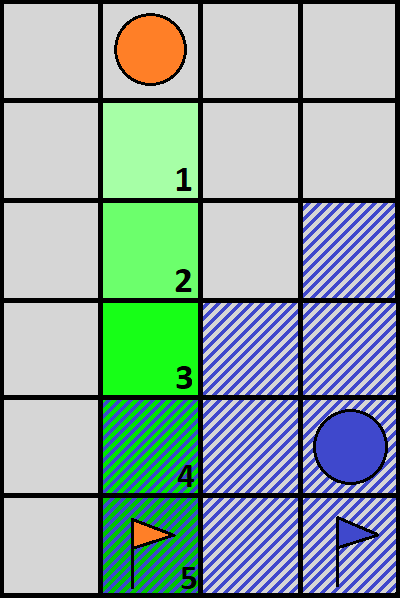
\includegraphics[width=\textwidth]{img/two-agents.png}
%\caption{}
%\label{fig:two_agents}
%\end{subfigure}
%\hfill
%\begin{subfigure}{0.3\columnwidth}
%\centering
%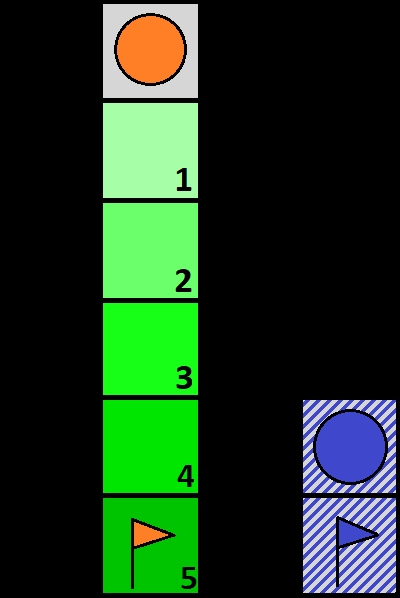
\includegraphics[width=\textwidth]{img/two-agents-path.png}
%\caption{}
%\label{fig:two_agents_path}
%\end{subfigure}
%\hspace{0.8cm}
%\caption{An instance with two agents, one with longer path allowing the other to move more freely.}
%\label{fig:two_agents_example}
%\end{figure}



Of course, this pruning does not maintain completeness in general. A simple counterexample can be seen in Figure~\ref{fig:m_counterexample}. The two agents want to swap their location (ie. their goal location is identical with the starting location of the other agent). To do this, the only solution is for both of them to travel to the right and use the top vertex to switch their position. %If we were to use our pruning technique, this would not be possible, making the example unsolvable.
To mitigate these instances,several strategies are proposed to change which vertices are pruned.

\begin{figure}[ht]
\centering
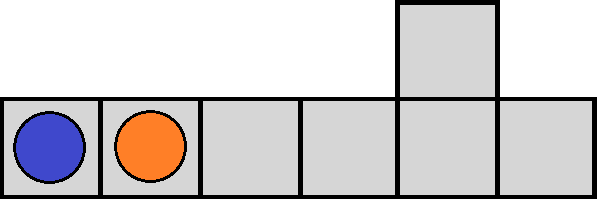
\includegraphics[width=0.45\columnwidth]{img/m_counterexample.png}
\caption{An instance with two agents that want to swap their positions.}
\label{fig:m_counterexample}
\end{figure}

%%% Local Variables:
%%% mode: latex
%%% TeX-master: "main"
%%% End:

\subsection{Solving Strategies}

%First, we start by explaining the solving strategies used in the initial study on the graph pruning technique [citation omitted].%~\cite{TODO}.

We will use the following notations. Let $SP_i$ be the vertices on a chosen shortest path for agent $a_i \in A$ (ie. a single shortest path from $s_i$ to $g_i$). The length of the path is $|SP_i|$. The union of vertices on the shortest paths of all agents is $SP_A = \bigcup_{a_i \in A} SP_i$. Note that for now for each agent we consider just one shortest path. If multiple shortest paths exist for an agent, one is chosen at random. Given this notation the lower bound on makespan of an instance $\inst = (G,A)$ can be written as $LB_{mks}(G,A) = \max_{a_i \in A} |SP_i|$. For short, we refer to such lower bound just by $LB$.

%\begin{figure}[ht]
%\centering
%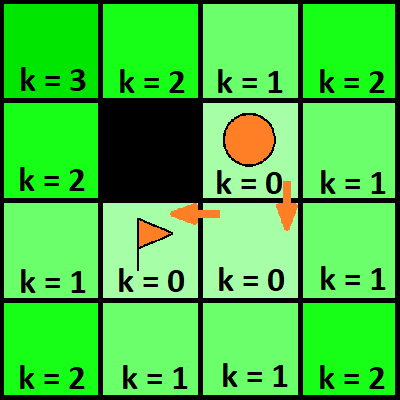
\includegraphics[width=0.37\columnwidth]{img/corridor.png}
%\caption{An instance with a single agent. Each vertex is labeled into which k-restricted graph it belongs.}
%\label{fig:corridor_width}
%\end{figure}

A \emph{k-restricted graph} $Gres_{k}^{SP_A}$ is a subgraph of $G$ containing only vertices $SP_A$ and vertices that are at most distance $k$ away from some vertex in $SP_A$. %, ie. $Gres_{k}^{SP_A} = \{v \in V \: | \: \exists u \in SP_A, \: dist(u,v) \leq k\}$.
Since we always fix $SP_A$, we write for simplicity only $Gres_k$. Note that $Gres_k \subseteq Gres_{k'}$ for $k \leq k'$. %An example of k-restricted graph can be seen in Figure~\ref{fig:corridor_width}. For a 0-restricted graph, only the shortest path is part of the graph. A 3-restricted graph is the whole initial graph in this case.

Since makespan optimal solution is found by iteratively increasing the makespan, we define a \emph{makespan-restricted} MAPF instance $\inst = (G,A,H)$. %This is the same problem as finding the solution for $\inst = (G,A)$ in makespan $H$.

The \emph{(k,m)-relaxation} of $\inst$ is the makespan-restricted MAPF instance
\[
  \mrelax{\inst}{k}{m} = (Gres_k,A,LB+m)
\]
This relaxation means that instead of the whole graph $G$ we consider only $Gres_k$ and we are finding a solution with extra makespan $m$ -- extra over the lower bound on makespan. Also note that $Gres_k$ is constructed such that $LB_{mks}(G,A) = LB_{mks}(Gres_k,A)$ for any $k$, therefore, we do not need to change the notation of $LB$.

We can build a partial order $\mrelaxle$ over the ($k$,$m$)-relaxations $\mrelax{\inst}{k}{m}$ such that 
\[
\mrelax{\inst}{k}{m} \mrelaxle \mrelax{\inst}{k'}{m'}
\]
\noindent if $k \leq k'$, $m\leq m'$ and $k+m < k'+m'$

There is an upper bound on $k$ such that for some $k_{max}$ we have $Gres_{k_{max}} = G$. There is also an upper bound on makespan for a given MAPF instance of $\mathcal{O}(V^3)$~\cite{pebble_motion}. %, however, in this paper we work only with solvable instances (this can be checked by polynomial-time algorithm) and we do not need to know the exact upper bound on makespan.
For an example, assume that $k_{max}=3$ and $m_{max}=2$. Then, Figure~\ref{fig:example-relax} depicts the space of possible relaxations induced by $\mrelaxle$. Note that the partial ordering forms a lattice.

\begin{figure}[h]
  \centering
  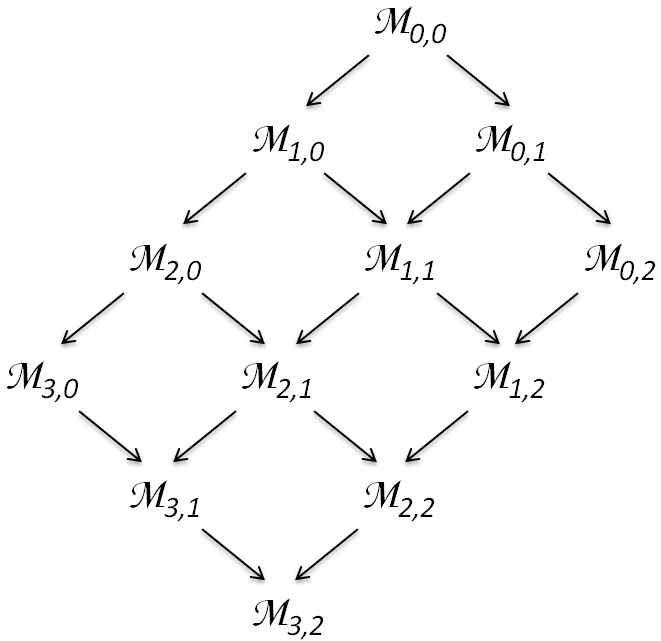
\includegraphics[width=0.65\columnwidth]{img/km_relax}
  \caption{Instance relaxations for \(k_{max}=3, m_{max}=2\).}
  \label{fig:example-relax}
\end{figure}

The generic algorithm to solve MAPF using the relaxed instances is as follows. First, we build an initial ($k$,$m$)-relaxation and we iteratively change $k$ and $m$ until the instance is solvable. This corresponds to a traversal of the lattice formed by the partial ordering $\mrelaxle$. Note that the shortest path for each agent is fixed for all of the iterations. Next we identify four reasonable traversals.

%\begin{algorithm}
%\caption{Generic algorithm solving MAPF using relaxation.}
%\label{alg:relaxation}
%\begin{algorithmic}
%\Function{Generic MAPF relaxation}{$\inst=(G,A)$}
% \State $LB = \max_{a_i \in A} |SP_i|$
% \State $(k,m) \gets Initial\_Candidate()$
% \While{not solve\_MAPF($\mrelax{\inst}{k}{m}$)}
%  \State $(k,m) \gets Relax()$
% \EndWhile
% \State \Return $LB + m$
%\EndFunction
%\end{algorithmic}
%\end{algorithm}


\subsubsection{Baseline Strategy}

The classical approach to solving MAPF makespan optimally can be expressed in the relaxed instances as follows. We start with an initial candidate of $k_{max}$ (ie. the whole graph $G$) and $m=0$. If the relaxed instance is unsolvable, only the additional makespan is increased as $m=m+1$. %In terms of the Figure~\ref{fig:example-relax}, the first solved relaxation is $\mrelax{\inst}{3}{0}$ and then we are moving only to the right-hand side. 
We shall refer to this strategy as \emph{baseline} or \ssb{} for short.

\begin{prop}\label{prop:baseline}
If a MAPF instance $\inst$ has a solution, \emph{baseline} strategy finds an optimal solution.
\end{prop}

%\begin{proof}
%Since $\inst$ has a solution, there needs to be an optimal solution with some makespan $H$ such that $LB \leq H$. The \emph{baseline} strategy will try all of the possible makespans $LB, \dots, H$, with $H$ being the first solvable.
%\end{proof}

\subsubsection{Makespan-add Strategy}

The first smarter solution is to keep only the vertices on the shortest paths and the immediately adjacent ones. The initial candidate is $k=1$ and $m=0$. Otherwise, the strategy is the same as the baseline strategy -- if the relaxed instance is unsolvable, we increase $m = m+1$ while the $k$ is never changed. We refer to this strategy as \emph{makespan-add} or \ssm{} for short.

\begin{prop}
\emph{Makespan-add} strategy is both suboptimal and incomplete.~\cite{AAMAS_corridors}
\end{prop}

%\begin{proof}
%For a simple example where \emph{makespan-add} cannot find a solution recall Figure~\ref{fig:m_counterexample}. No matter how the initial constant of $k$ is set, we can create a graph where the extra vertex needed for the two agents to swap is not part of $Gres_k$.

%For an example where \emph{makespan-add} finds a suboptimal solution see figure~\ref{fig:p_counterexample} with blue agent choosing the blue path. In this case \emph{makespan-add} needs to increase $m$ two times to find a solution, while it would be possible to find a solution in $LB$ steps if the vertices of the black path were included.
%\end{proof}


On the other hand, in most cases, this simple strategy can find a solution, and due to the great reduction of vertices of the graph, the solution may be found quickly. We choose to start with $k=1$ rather than $k=0$ to increase the probability for a solution to exist while keeping the number of vertices to a minimum.

%In terms of Figure~\ref{fig:example-relax}, the strategy first moves to the left once and then only to the right. 


\subsubsection{Prune-and-cut Strategy}

The previous strategies either use unnecessary large restricted graph or do not guarantee to find a solution. Strategy \emph{prune-and-cut} (\ssp{} for short) guarantees both completeness and optimality. We start with initial candidate $k=0$ and $m=0$. In case the relaxed instance is unsolvable, we cannot be sure if the reason is the restriction on $k$ or on $m$. However, since we do not want to overestimate $m$, we first need to increase $k$ potentially up to $k_{max}$. Once a restricted instance $\mrelax{\inst}{k_{max}}{m}$ is unsolvable, we are sure that $m$ needs to be increased. %Since we proved that we require at least $m+1$ extra makespan, 
we can optimistically assume that the whole $Gres_{k_{max}}$ is not needed and we restrict the graph back to $k=0$ producing $\mrelax{\inst}{0}{m+1}$.


\begin{prop}
If a MAPF instance $\inst$ has a solution, \emph{prune-and-cut} strategy finds an optimal solution.~\cite{AAMAS_corridors}
\end{prop}

%\begin{proof}
%Before $m$ is increased, we always check if there is a solution using the original $G$. The rest of the proof is the same as for Proposition~\ref{prop:baseline}.
%\end{proof}


%During our initial experiments, it turned out that the whole $Gres_{k_{max}}$ is usually not necessary. Therefore, increasing $k$ by 1 each time may prove inefficient, since most of the calls are unsolvable and we just need to prove that we can increase $m$. For this reason we increase $k$ by powers of 2 (ie. $k = k+1, k=k+2, k=k+4, \dots$).

%Another implementation improvement is to not increase up to $k_{max}$ but rather to some $k \leq k_{max}$ that produces $Gres_{k}$ that includes all of the vertices reachable in given $LB + m$ by some agent. This information can be obtained by the preprocessing.

%The visualization of solver calls of the \emph{prune-and-cut} strategy over the lattice can be seen in Figure~\ref{fig:example-relax-P}.

%\begin{figure}[ht]
%\centering
%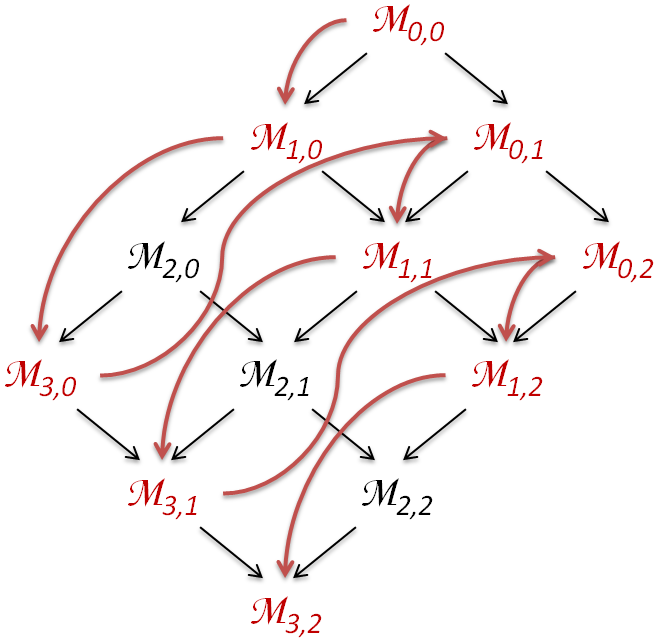
\includegraphics[width=0.75\columnwidth]{img/Pstrat_km_relax.png}
%\caption{The traversal of the lattice by strategy \emph{prune-and-cut}. The highlighted relaxed instances are being solved.}
%\label{fig:example-relax-P}
%\end{figure}


\subsubsection{Combined Strategy}

The drawback of the \emph{prune-and-cut} strategy is that in the case the makespan needs to be increased, we first increase $k$ up to $k_{max}$ before increasing $m$. To mitigate this problem, we present the \emph{combined} strategy (\ssc{} for short). The initial candidate is again $k=0$ and $m=0$. If the relaxed instance is unsolvable, we increase both $k=k+1$ and $m=m+1$ at the same time. This way, we save the number of calls to the solver because we do not need to explore all of the possible reductions in the $k$ direction. On the other hand, this strategy is no longer optimal. Figure~\ref{fig:p_counterexample} with blue agent choosing the blue path is such an example.

\begin{prop}
If a MAPF instance $\inst$ has a solution, \emph{combined} strategy is guaranteed to find a solution (completeness) but not necessarily an optimal one.~\cite{AAMAS_corridors}
\end{prop}

%\begin{proof}
%If it is necessary to use all of the vertices in the graph $G$ to find a solution, \emph{combined} strategy will eventually increase $k$ up to $k_{max}$ since $k_{max}$ is a finite number. However, in doing so, it may overestimate the $m$ needed. Figure~\ref{fig:p_counterexample} with blue agent choosing the blue path is again such an example.
%\end{proof}

\begin{figure}[ht]
\centering
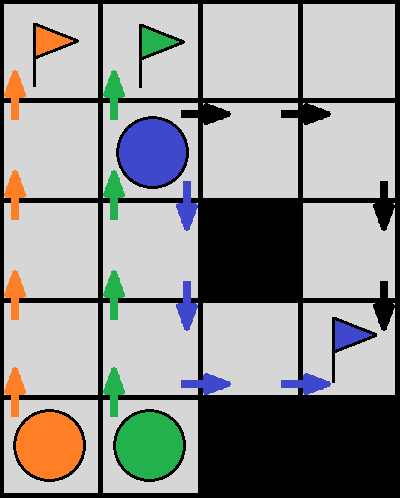
\includegraphics[width=0.3\columnwidth]{img/p_counterexample.png}
\caption{An example instance where the blue agent has two choices of the shortest path. If the blue path is chosen, the proposed strategies perform worse.}
\label{fig:p_counterexample}
\end{figure}



%%% Local Variables:
%%% mode: latex
%%% TeX-master: "main"
%%% End:


\section{Choosing the Shortest Paths}
\label{sec:SP}

The described strategies (except for \emph{baseline}) may suffer from a poor choice of the initial shortest path for each agent. See the example in Figure~\ref{fig:p_counterexample}. The blue agent has two possible shortest paths. If the algorithm by random chooses the blue path, none of the sophisticated strategies can solve the relaxed instance in the first solver call. \emph{Makespan-add} would find a suboptimal solution with makespan $LB+2$, \emph{prune-and-cut} would require to increase $k$ two times to be able to use the black path, and \emph{combined} strategy would also find a suboptimal solution with makespan $LB+2$.

This issue can be mitigated by including all of the vertices on all of the possible shortest paths into the $\mathit{Gres}_{k}$, however, this goes against the logic of the motivational example in Figure~\ref{fig:diagonal_example}. Hence, we try to identify approaches to choose more than just one of the shortest paths to improve the strategies.

Since the choice of the shortest paths acts as a preprocessing stage, we aim for fast heuristic techniques. For this reason, each agent is treated individually, without considering the interference with shortest paths of the other agents. We propose the following four sensible approaches to pick which vertices should be included in the initial restricted graph $\mathit{Gres}_{0}$. All of the described strategies, then, work the same as was described in the previous section.
%
\begin{figure*}[ht]
\centering

\begin{subfigure}[t]{0.99\columnwidth}
\centering
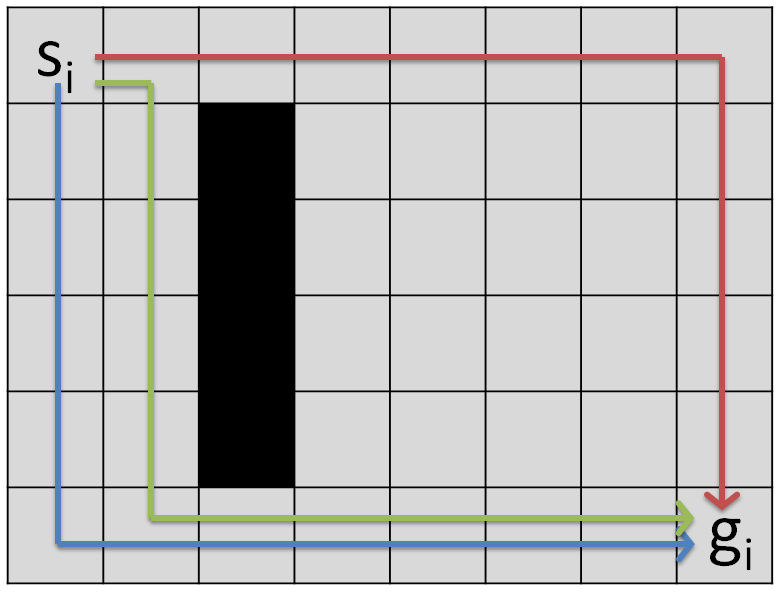
\includegraphics[width=0.45\columnwidth]{img/distant_wrong.PNG}
\caption{The greedy approach starting at $s_i$ chooses an undesirable green path due to the fact that it tries to make the path most divers (to the previously planned blue and red paths) from the start without the knowledge of the rest of the map.} %After passing the obstacle, the approach is forced to choose the same vertices as are on the blue path.}
\label{fig:distant_wrong}
\end{subfigure}
\hfill
\begin{subfigure}[t]{0.99\columnwidth}
\centering
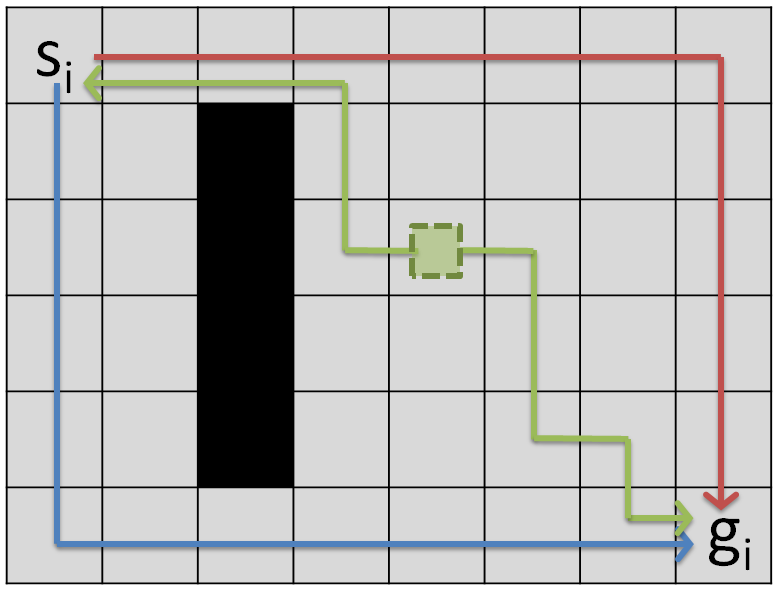
\includegraphics[width=0.45\columnwidth]{img/distant_ok.PNG}
\caption{By choosing a different starting location, the greedy algorithm finds a better green path than in Figure~\ref{fig:distant_wrong}. In this example there are multiple possible starting locations, each equally good. If this happens, one is chosen at random.}
\label{fig:distant_ok}
\end{subfigure}
\caption{An example showing the drawback of finding the shortest path greedily from the the starting location $s_i$. This issue can be fixed by choosing different starting vertex. The green path is chosen after red and blue paths.}
\label{fig:distant}
\end{figure*}

% \subsection{Single Path}
\textbf{Single Path.}
First, we use the same approach as in the original study~\cite{AAMAS_corridors}.
For each agent, we choose a single random shortest path. The restricted graph $\mathit{Gres}_{0}$ is induced by $SP_A = \bigcup_{a_i \in A} SP_i$. Recall that $SP_i$ are the vertices on the shortest path for agent $a_i$. We refer to this approach as \emph{single-path} or \pss{} for short.

% \subsection{All Paths}
\textbf{All Paths.}
The second approach is on the other end of the spectrum. Instead of just one shortest path, we consider all vertices on all shortest paths of a given agent. Formally, we write $SP_i^{\mathit{All}} = \{ v \in V \: | \: \mathit{dist}(s_i,v) + \mathit{dist}(v,g_i) = |SP_i|\}$ meaning all vertices whose distance from start location plus the distance to goal location equals the distance of a shortest path. The restricted graph $\mathit{Gres}_{0}$ is induced by $SP_A^{\mathit{All}} = \bigcup_{a_i \in A} SP_i^{\mathit{All}}$.

Note that while there may be many different shortest paths as discussed in Figure~\ref{fig:diagonal_example}, the number of vertices on those paths is much smaller. For the creation of the restricted graph, we are interested only in the vertices, the specific path is decided by the underlying solver. Finding all of the vertices on all of the shortest paths can be done by performing a breath-first search from the start and goal of the agent and checking for the condition in the definition of $SP_i^{\mathit{All}}$. We refer to this approach as \emph{all-paths} or \psa{} for short.




% \subsection{Random Paths}
%
\textbf{Random Paths.}
Instead of considering one or all possible paths, we aim to pick vertices that are part of just some subset of all paths. First, we need to set a number of paths to consider. Note that based on the given map and the start and goal locations of each agent, there is a wide variety of the number of shortest paths. Instead of selecting a magic constant, we propose to find $\frac{|SP_i^{\mathit{All}}|}{|SP_i|}$ shortest paths for agent $a_i$ and consider the union of vertices on those. If there is a unique shortest path, by using the formula we correctly consider just the one shortest path, while on an empty $N \times N$ grid (such as in Figure~\ref{fig:diagonal_example}), we are considering $\frac{N}{2}$ paths.

The next proposed approach picks the specified number of shortest paths randomly. We do this by a random walk starting at $s_i$ moving only over vertices from $SP_i^{\mathit{All}}$ in the correct direction. We know the correct direction based on the distance from $s_i$ and $g_i$ computed by BFS (we need to perform the two BFS in order to determine $SP_i^{\mathit{All}}$). The random walk is biased to prefer vertices that are not yet used for a given agent. By doing this for all agents we get $SP_A^{Rand} = \bigcup_{a_i \in A} SP_i^{Rand}$. We refer to this approach as \emph{random-paths} or \psr{} for short.




% \subsection{Distant Paths}
%
\textbf{Distant Paths.}
The drawback of \emph{random-paths} it that there is no guarantee on the properties of the chosen shortest paths. The idea of using more than one shortest path is to allow the underlying solver to navigate the agent through a different region of the map to avoid possible conflicts. However, by choosing random paths, we may produce paths that share many vertices or are in close proximity to each other, both of which are undesirable.

We want to find \emph{diverse} and \emph{distant} paths. There is a polynomial-time algorithm to find diverse shortest paths~\cite{diverse}. In this case, diverse means paths that share the least amount of edges (or vertices). By using this algorithm, it may be the case that we find paths as shown in Figure~\ref{fig:diverse}. On the other hand, there is also a research dealing with finding the most diverse near-shortest paths~\cite{distant}, in which case the paths are supposed to be the greatest distance from each other. Note that both studies use the term distant with different meaning. In our paper, we are using \emph{diverse} for different paths and \emph{distant} for path with distance between them. The downside of the the second referred study is that the paths found are not optimal and also the problem itself is NP-Hard, which is not a desirable trait for a preprocessing function.

\begin{figure}[hb]
\centering
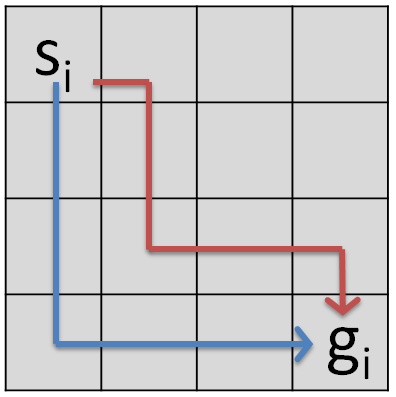
\includegraphics[width=0.25\columnwidth]{img/diverse.PNG}
\caption{Possible shortest paths from $s_i$ to $g_i$ found by the diverse shortest paths algorithm~\cite{diverse}.}
\label{fig:diverse}
\end{figure}


Our proposed approach is heuristic. Again, we build the paths over the vertices from $SP_i^{\mathit{All}}$, gradually creating $SP_i^{\mathit{Dist}}$. At each step, we try to add a new vertex to the currently build path and if there are multiple choices, we pick one that maximizes the minimal distance to all of the vertices currently in $SP_i^{\mathit{Dist}}$ (see Figure~\ref{fig:distant_choose} for an example).
%
\begin{figure}[ht]
\centering
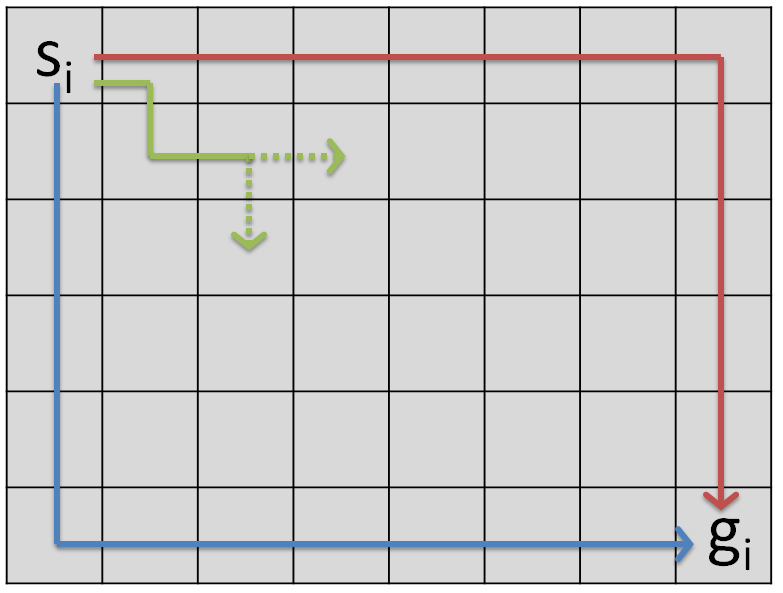
\includegraphics[width=0.45\columnwidth]{img/distant_choose.PNG}
\caption{The gradual building of $SP_i^{\mathit{Dist}}$ from $s_i$ to $g_i$ by a greedy approach. The currently build green path has a choice. Moving downward will be chosen since it maximizes the distance to the already chosen paths.}
\label{fig:distant_choose}
\end{figure}
%
Since this is just a heuristic, there are examples that make us choose an undesirable path because the approach greedily chose the next vertex on the path without knowledge of the rest of the map. Such example can be seen in Figure~\ref{fig:distant_wrong}. To mitigate this, we start to build the path from a different vertex from the set $SP_i^{\mathit{All}}$ rather than from $s_i$. The first path is build the same as $SP_i$, for the latter paths, we choose a vertex $v$ such that it maximizes the minimal distance to all of the vertices currently in $SP_i^{\mathit{Dist}}$. This way we need to build the path both from $v$ to $s_i$ and from $v$ to $g_i$. Using this approach we find a much more desirable path for the example in Figure~\ref{fig:distant_wrong} with the result shown in Figure~\ref{fig:distant_ok}. We refer to this approach as \emph{distant-paths} or \psd{} for short.

%%% Local Variables:
%%% mode: latex
%%% TeX-master: "main"
%%% End:

\section{Experimental Evaluation}

\def\arraystretch{1.1}

% Please add the following required packages to your document preamble:
% \usepackage{multirow}
% \usepackage{graphicx}
\begin{table*}[ht]
\centering
\resizebox{\textwidth}{!}{%
\begin{tabular}{ll|l|llll|llll|llll}
                                                                                                         &               & \multicolumn{1}{c|}{\multirow{2}{*}{\ssb}} & \multicolumn{4}{c|}{\ssp}                                      & \multicolumn{4}{c|}{\ssc}                                       & \multicolumn{4}{c}{\ssm}                                      \\
                                                                                                         	&	 type          	&	 \multicolumn{1}{c|}{}                      	&	 \pss            	&	 \psa          	&	 \psr          	&	 \psd         	&	 \pss            	&	 \psa          	&	 \psr          	&	 \psd          	&	 \pss          	&	 \psa          	&	\psr	&	 \psd          	\\	\hline
\multicolumn{1}{l|}{\multirow{4}{*}{\begin{tabular}[c]{@{}l@{}}Used\\ vertices\end{tabular}}}            	&	 \emph{empty}  	&	1	&	 \textbf{0.14}   	&	0.23	&	0.21	&	0.23	&	 \textbf{0.15}   	&	0.24	&	0.22	&	0.23	&	0.19	&	0.24	&	0.23	&	0.24	\\
\multicolumn{1}{l|}{}                                                                                    	&	 \emph{maze}   	&	1	&	 \textbf{0.18}   	&	0.2	&	 \textbf{0.18} 	&	0.19	&	 \textbf{0.20}   	&	0.22	&	0.21	&	0.21	&	0.22	&	0.22	&	0.22	&	0.22	\\
\multicolumn{1}{l|}{}                                                                                    	&	 \emph{random} 	&	1	&	 \textbf{0.19}   	&	0.27	&	0.24	&	0.25	&	 \textbf{0.22}   	&	0.3	&	0.28	&	0.29	&	0.25	&	0.31	&	0.3	&	0.31	\\
\multicolumn{1}{l|}{}                                                                                    	&	 \emph{room}   	&	1	&	 \textbf{0.21}   	&	0.24	&	0.22	&	0.22	&	 \textbf{0.23}   	&	0.27	&	0.25	&	0.25	&	0.24	&	0.29	&	0.27	&	0.28	\\	\hline
\multicolumn{1}{l|}{\multirow{4}{*}{\begin{tabular}[c]{@{}l@{}}Solved\\ instances\end{tabular}}}         	&	 \emph{empty}  	&	0.78	&	 \textbf{0.99}   	&	0.81	&	0.84	&	0.82	&	 \textbf{1.00}   	&	0.81	&	0.84	&	0.82	&	0.87	&	0.81	&	0.82	&	0.8	\\
\multicolumn{1}{l|}{}                                                                                    	&	 \emph{maze}   	&	0.85	&	0.87	&	 \textbf{0.88} 	&	0.87	&	0.87	&	 \textbf{0.98}   	&	0.97	&	0.97	&	 \textbf{0.98} 	&	0.94	&	0.94	&	0.94	&	0.94	\\
\multicolumn{1}{l|}{}                                                                                    	&	 \emph{random} 	&	0.79	&	 \textbf{0.91}   	&	0.82	&	0.84	&	0.84	&	 \textbf{1.00}   	&	0.89	&	0.92	&	0.91	&	0.93	&	0.87	&	0.89	&	0.88	\\
\multicolumn{1}{l|}{}                                                                                    	&	 \emph{room}   	&	0.8	&	 \textbf{0.83}   	&	0.81	&	0.82	&	0.82	&	 \textbf{0.97}   	&	0.92	&	0.95	&	0.94	&	0.89	&	0.89	&	0.89	&	0.89	\\	\hline
\multicolumn{1}{l|}{\multirow{5}{*}{$\sum$ IPC}}                                                         	&	 \emph{empty}  	&	874.6	&	 \textbf{1930.5} 	&	1312.8	&	1081.7	&	1086.3	&	 \textbf{2395.2} 	&	1276.5	&	1406.7	&	1324.4	&	1517.9	&	1275.8	&	1312.5	&	1279.2	\\
\multicolumn{1}{l|}{}                                                                                    	&	 \emph{maze}   	&	890.1	&	 \textbf{1153.2} 	&	1123.6	&	1128.3	&	1143.3	&	 \textbf{1775.5} 	&	1633.8	&	1752.8	&	1754	&	1475.7	&	1452.6	&	1470.5	&	1466.1	\\
\multicolumn{1}{l|}{}                                                                                    	&	 \emph{random} 	&	886	&	 \textbf{1668.0} 	&	1110.2	&	1049.9	&	1102.3	&	 \textbf{2275.5} 	&	1422.4	&	1594.6	&	1551.5	&	1560.7	&	1300.3	&	1374.2	&	1324.4	\\
\multicolumn{1}{l|}{}                                                                                    	&	 \emph{room}   	&	877.3	&	 \textbf{1386.4} 	&	1007.5	&	1191.6	&	1179.5	&	 \textbf{2078.3} 	&	1594.5	&	1850.6	&	1828.7	&	1474	&	1382.6	&	1461.9	&	1442	\\	\cline{2-15}
\multicolumn{1}{l|}{}                                                                                    	&	 total         	&	3527.9	&	 \textbf{6138.1} 	&	4554.1	&	4451.6	&	4511.4	&	 \textbf{8524.5} 	&	5927.2	&	6604.6	&	6458.6	&	6028.4	&	5411.3	&	5619.2	&	5511.6	\\	\hline
\multicolumn{1}{l|}{\multirow{4}{*}{\begin{tabular}[c]{@{}l@{}}Solved\\ optimally\end{tabular}}}         	&	 \emph{empty}  	&	 -                                          	&	 -               	&	 -             	&	 -             	&	 -            	&	0.93	&	 \textbf{1.00} 	&	 \textbf{1.00} 	&	 \textbf{1.00} 	&	 \textbf{1.00} 	&	 \textbf{1.00} 	&	\textbf{1.00}	&	 \textbf{1.00} 	\\
\multicolumn{1}{l|}{}                                                                                    	&	 \emph{maze}   	&	 -                                          	&	 -               	&	 -             	&	 -             	&	 -            	&	0.91	&	 \textbf{0.94} 	&	0.92	&	0.92	&	0.92	&	0.93	&	0.93	&	0.93	\\
\multicolumn{1}{l|}{}                                                                                    	&	 \emph{random} 	&	 -                                          	&	 -               	&	 -             	&	 -             	&	 -            	&	0.89	&	 \textbf{0.97} 	&	0.95	&	0.96	&	0.86	&	0.91	&	0.91	&	0.91	\\
\multicolumn{1}{l|}{}                                                                                    	&	 \emph{room}   	&	 -                                          	&	 -               	&	 -             	&	 -             	&	 -            	&	0.86	&	 \textbf{0.93} 	&	0.91	&	0.92	&	0.76	&	0.86	&	0.85	&	0.85	\\	\hline
\multicolumn{1}{l|}{\multirow{4}{*}{Conflicts}}                                                          	&	 \emph{empty}  	&	133	&	 \textbf{97}     	&	148	&	131	&	136	&	 \textbf{111}    	&	147	&	141	&	142	&	139	&	148	&	146	&	148	\\
\multicolumn{1}{l|}{}                                                                                    	&	 \emph{maze}   	&	2457	&	 \textbf{1239}   	&	1804	&	1274	&	1265	&	3101	&	 \textbf{2969} 	&	3120	&	3143	&	3361	&	3482	&	3443	&	3354	\\
\multicolumn{1}{l|}{}                                                                                    	&	 \emph{random} 	&	206	&	193	&	195	&	174	&	 \textbf{173} 	&	 \textbf{218}    	&	235	&	234	&	227	&	448	&	458	&	460	&	459	\\
\multicolumn{1}{l|}{}                                                                                    	&	 \emph{room}   	&	1007	&	402	&	313	&	270	&	 \textbf{289} 	&	1642	&	1414	&	1513	&	1423	&	1525	&	 \textbf{1400} 	&	1527	&	1545	\\	\hline
\multicolumn{1}{l|}{\multirow{4}{*}{\begin{tabular}[c]{@{}l@{}}Constraints\\ {[millions]}\end{tabular}}} 	&	 \emph{empty}  	&	 \textbf{4.7}                               	&	7.3	&	5.1	&	5.9	&	5.2	&	7.4	&	5.1	&	6	&	5.2	&	6	&	 \textbf{5.0}  	&	5.2	&	 \textbf{5.0}  	\\
\multicolumn{1}{l|}{}                                                                                    	&	 \emph{maze}   	&	 \textbf{6.0}                               	&	6.1	&	6.4	&	6	&	6.2	&	 \textbf{6.4}    	&	6.8	&	6.5	&	6.6	&	6.8	&	6.8	&	6.8	&	6.8	\\
\multicolumn{1}{l|}{}                                                                                    	&	 \emph{random} 	&	 \textbf{5.4}                               	&	5.9	&	6	&	6	&	6	&	6	&	6.1	&	6.1	&	6.1	&	6.1	&	 \textbf{5.8}  	&	6	&	 \textbf{5.8}  	\\
\multicolumn{1}{l|}{}                                                                                    	&	 \emph{room}   	&	 \textbf{4.8}                               	&	5.4	&	5.6	&	5.4	&	5.4	&	 \textbf{5.7}    	&	5.9	&	5.8	&	 \textbf{5.7}  	&	 \textbf{5.7}  	&	5.9	&	5.9	&	5.9
\end{tabular}%
}
\caption{Ratio of used vertices, ratio of solved instances,  sum of IPC score, ratio of instances solved optimally, average number of conflicts, and average number of constraints. The results are split by the map type. Strategies are \emph{baseline} (\ssb{}), \emph{prune-and-cut} (\ssp{}), \emph{makespan-add} (\ssm{}), and \emph{combined} (\ssc{}). Approaches to choosing shortest paths are \emph{single-path} (\pss), \emph{all-paths} (\psa), \emph{random-paths} (\psr), and \emph{distant-paths} (\psd).}
\label{tab:results}
\end{table*}


To test and compare the proposed strategies in combination with approaches to creating the restricted graph, we set up experiments. The full implementation and results are available at \url{https://github.com/potassco/mapf-subgraph-system}. For the ASP-based solver, we used the grounding-and-solving system \emph{clingo}~\cite{PotasscoUserGuide19,karoscwa20a} version~\(5.5.2\). We ran the experiments on an Intel Xeon E5-2650v4 under Debian GNU/Linux~9, with each instance limited to 300s processing time and 28 GB of memory.


% \subsection{Instances}
%
The instances used in our experiments are based on commonly used benchmark instances available online~\cite{stern2019mapfVarians}. We chose different sizes of maps -- \emph{small} (32 by 32), \emph{medium} (64 by 64), and \emph{large} (128 by 128) and different structures of the impassable obstacles in the map with the following types -- \emph{empty}, \emph{maze}, \emph{random}, and \emph{room}. % (see Figure~\ref{fig:maps} for reference). Unfortunately, some of the combinations of size and type were not available in the benchmark set, therefore, we had to create our own following the structure of the existing maps.

%\begin{figure}[ht]
%\centering
%
\includegraphics[width=0.75\columnwidth]{img/maps_32.png}
%\caption{Types of maps used in the experimental evaluation. From left to right: \emph{maze}, \emph{random}, and \emph{room}.}
%\label{fig:maps}
%\end{figure}

For the placement of the agents (called \emph{scenarios}), we used the available scenarios. % from the benchmark sets or, if not present, created our own. For each map, we used 5 different scenarios.
Furthermore, we created new scenarios for each map such that the distance from start to goal of each agent is similar and the paths of the agents need to cross more often. We did this because the makespan optimal solution for the random scenarios rarely differs from the lower bound. %This is caused by one of the agents having a much longer path than the others leaving them with enough time to solve any conflicts.
The behavior of the strategies may be gravely affected by many conflicts and the need to increase the makespan.% We are also using 5 different scenarios with this setting.

The intended way to use the benchmark set is to create an instance of MAPF from a map and a number of agents from a scenario. If the instance is solved in the given time limit, an additional agent from the same scenario is added and thus a new MAPF instance is produced. Once the instance cannot be solved in the time limit, it is reasoned that increasing further the number of agents cannot make the instance solvable. We are aware that using a reduction-based solver, this may not always hold. Also, some of the strategies may benefit from additional agents which change the restricted graph. However, these cases are extremely rare and therefore, we decided to use the benchmark as intended.


%\subsection{Results}
%
Table~\ref{tab:results} shows the results for all of the strategies and approaches to creating the restricted graph. Note that the \emph{baseline} strategy \ssb{} considers the whole map, therefore we do not use any of the four approaches. The strategies \ssb{} and \ssp{} are optimal, therefore, we consider them separately opposed to the suboptimal strategies \ssc{} and \ssm{}. The best result for both optimal and suboptimal strategies on each line is highlighted. We present the results divided by the type of the map regardless of the size. This representation shows nicely the difference between the approaches to creating the restricted graph. For more detailed results, we include much more detailed tables in the supplementary materials.

First, we examine the average number of vertices used by each approach. In the table, the number indicates the ratio of used vertices to the total number of vertices. Since \ssb{} always uses the whole map, the ratio is $1$. We can see that \pss{} uses the least number of vertices in all cases, on the other hand, \psa{} uses the most and \psd{} and \psr{} use about the same. This result is not surprising since it is based on the number of paths used by each approach. However, we can also see that the difference is much bigger on opened maps (such as \emph{empty}) and much smaller on very restrictive maps (such as \emph{maze}), meaning that in the latter case there are not many different shortest paths for the agents to choose from. There is also a clear order in terms of the strategies with \ssp{} using the least, \ssc{} using more, and \ssm{} using even more vertices on average.

Examining the number of solved instances (ratio of solved to all instances -- 2544 for \emph{empty}, 1956 for \emph{maze}, 2418 for \emph{random}, 2357 for \emph{room}), we see that the most successful combination is \ssp{} + \pss{} for the optimal setting and \ssc{} + \pss{} for the suboptimal. Again, the difference across the approaches to choosing the shortest paths is least prominent on \emph{maze} maps, however, on the other types, the order is clear. The \pss{} is the most successful, \psd{} and \psr{} performing about the same, while \psa{} performs the worst. The \emph{baseline} \ssb{} performs worse than any other used combination.
Similar results can be seen when exploring the IPC score~\footnote{introduced at International Planning Competition.} (Computed as 0 if the solver did not finish in time, otherwise as $\frac{\textit{min. time}}{\textit{solver time}},$ where \textit{min. time} is the time it took the fastest solver and \textit{solver time} is the time it took the solver in question. The score ranges from 0 to 1, where the bigger the number the better. The scores of all instances are summed.) For the \ssp{} strategy the \psa{} approach performs better than \psd{} and \psr{}, meaning that while it did not solve more instances, the instances it managed to solve were solved faster. For the other strategies, the order remains the same as with the number of solved instances. It is unsurprising that the suboptimal strategies achieved a better score that the optimal \ssp{}.

We argue that these results stem from the number of used vertices. By exploring the ASP solver, we see that for all strategies and all additional shortest path approaches, the number of conflicts stays mostly within the same order of magnitude as for \pss{}. Hence, ASP search difficulty remains unchanged.
However, compared to \pss{}, the other approaches add more vertices to the restricted graph to consider and, in consequence, this increases the grounding time of \emph{clingo} which, in turn, leads to more timeouts.
%esp. for instances that finished close to 300s, for \pss{}.

The new shortest path approaches reduce the size of the internal problem specification in terms of the number of constraints.
We conjecture that since the new approaches generally select multiple (and more likely exclusively usable by one agent) vertices for the restricted graph, the amount of constraints encoding possible agent collisions is reduced. However, as mentioned above, this has no significant impact on the search complexity.

We also explore the quality of the solutions produced by the suboptimal strategies. The ratio of instances solved optimally is again shown in Table~\ref{tab:results}. Strategy \ssc{} is more often optimal compared to \ssm{}. This time, we can see the benefit of adding extra vertices to the restricted graph. The most often optimal approach is \psa{} closely followed by \psr{} and \psd{}, while \pss{} achieved the worst results. The difference is again less prominent on \emph{maze} maps.

%%% Local Variables:
%%% mode: latex
%%% TeX-master: "main"
%%% End:

\section{Conclusion}

We extended the study on pruning maps to increase the efficiency of reduction-based MAPF solvers. In the original paper, only one random path was chosen for each agent to build a restricted graph. Conversely, in this paper, we proposed several approaches to choosing multiple different paths for each agent, providing the underlying solver with more choices. In theory, this should make it possible for the agents to avoid collisions more easily. In our experiments, we found that this rarely happens and that it is more beneficial to provide the solver with just one random path making the relaxed instances simpler for the cost of possibly having to solve more relaxations. Thus, we showed that the original approach is justified, a result that is lacking in the original study.
%
On the other hand, we also showed that providing the agents with more possible paths leads more often to an optimal solution when using one of the suboptimal strategies.
%
%%% Local Variables:
%%% mode: latex
%%% TeX-master: "main"
%%% End:


%\vfill
\section*{\uppercase{Acknowledgements}}
Research is supported by
project P103-19-02183S of the Czech Science Foundation, % may be deleted
the Czech-USA Cooperative Scientific Research Project LTAUSA19072, and
DFG grant SCHA 550/15, Germany.


\bibliographystyle{apalike}
{\small
\bibliography{example}}


\end{document}

